\documentclass[12pt]{report}

\usepackage[letterpaper, margin=1truein, footskip=.25in, twoside]{geometry}
\usepackage[utf8]{inputenc}
\usepackage[english]{babel}

\usepackage{setspace}
\doublespacing

% Header and footer
\usepackage{fancyhdr}
\pagestyle{fancy}
\fancyhead{}
\fancyhead[RO,LE]{\thepage}
\fancyhead[RE]{\it\leftmark}
\fancyhead[LO]{\it\rightmark}
\fancyfoot{}

% Figures and images
\usepackage{graphicx}
\graphicspath{ {images/} }
\usepackage{color}
\usepackage[font={small,it}]{caption}
\usepackage{epsfig}
\usepackage{epstopdf}

% Make references clickable
\usepackage{hyperref}

% Custom Package with commands and common packages
\usepackage{my_package}

% Theorem environments
\usepackage{amsthm}
\theoremstyle{plain}
\newtheorem{thm}{Theorem}[section]
\newtheorem{lem}[thm]{Lemma}
\newtheorem{prop}[thm]{Proposition}
\newtheorem{cor}{Corollary}[section]
\newtheorem{subclaim}{Claim}[subsubsection]

\theoremstyle{definition}
\newtheorem{defn}{Definition}[section]
\newtheorem{conj}{Conjecture}[section]
\newtheorem{exmp}{Example}[section]

\theoremstyle{remark}
\newtheorem*{rem}{Remark}
\newtheorem*{conv}{Convention}


\begin{document}

% --- Title, Abstract, and Acknowledgements ---
\begin{titlepage}
   \begin{center}
       \vspace*{\fill}
       {GRAPH CONFIGURATION SPACES AND BRAID GROUPS}
 
       \vspace{1cm}
 
       A THESIS\\
       SUBMITTED TO THE GRADUATE SCHOOL\\
       IN PARTIAL FULFILLMENT OF THE REQUIREMENTS\\
       FOR THE DEGREE\\
       MASTER OF SCIENCE\\
       BY\\
       ZACH WILCHER\\
       DR. JUSTIN MURRAY - ADVISOR
 
       \vspace{1 cm}
 
       BALL STATE UNIVERSITY\\
       MUNCIE, INDIANA\\
       MAY 2026
       \vspace*{\fill}
   \end{center}
\end{titlepage}
\clearpage\shipout\null
\pagenumbering{roman}
\input{abstract.tex}
\input{acknowledgements.tex}
\tableofcontents
\clearpage\shipout\null
\pagenumbering{arabic}

% --- Content Chapters ---
\chapter{Configuration Spaces}
\section{Definitions and preliminary results}
% These definitions are presented in Abrams on page 10.
Given a topological space \(X\), the \(n\) point (topological) configuration space of \(X\) is
\(\Conf_n(X) = X^n - \Delta\) where \(\Delta\) is the diagonal in \(X^n\).

Treating a graph \(\Gamma\) as a topological space we can construct the
\(n\) point discretized or combinatorial configuration space \(\DConf_n(\Gamma)\) by 
% this diagonal needs elaboration.
removing a larger diagonal \(\Delta^{\square} = \{(e_1, \ldots, e_n) \mid x_i \cap x_j \neq \emptyset \text{ for some } i \neq j\}\)
from \(\Gamma^n\). Here \((e_1, \cdots, e_n)\) is any \(n\)-tuple of cells in \(\Gamma\).

Abrams showed in \cite{abrams2000configurationspaces} that \(\Conf_n(\Gamma)\) deformation retracts onto \(\DConf_n(\Gamma)\) and
that \(\DConf_n(\Gamma)\) is a cubical complex.
He also notes that any point in the
\(n\)-point configuration space is in one-to-one correspondence with a
collection of ``tokens'' placed on the graph. In this project, we will use a slightly different terminology and
and say ``particles'' instead of ``tokens.''

% TODO what is a cubical complex?
% make sure to define n-cubes and the gluing map

\begin{figure}[h!]
\centering
\begin{tikzpicture}
    \node (u1) at (2, 2) {\(u_1\)};
    \node (u2) at (4, 2) {\(u_2\)};
    \node (u3) at (3, 1) {\(u_3\)};
    \node (u4) at (3, 0) {\(u_4\)};
    \draw (u1) -- (u3);
    \draw (u2) -- (u3);
    \draw (u4) -- (u3);
\end{tikzpicture}
\caption{The \(Y\)-graph}
\label{fig:ygraph}
\end{figure}
Imagine \(2\) particles placed on the graph in \ref{fig:ygraph} at \(u_1\) and \(u_2\).  
In the topological configuration space, as the particle at \(u_1\) moves to \(u_3\)
the particle at \(u_2\) is free to simultaneously move to \(u_3\) as well. 
However, both particles would not be able to occupy the vertex \(u_3\) simultaneously.  
Compare this with the combinatorial configuration space, as the
particle at \(u_1\) moves to \(u_3\), the particle at \(u_2\) can not move at
all since the edges \(u_1 u_3\) and \(u_2 u_3\) intersect at \(u_3\) and points
with coordinates belonging to both edges are removed.

\begin{figure}[h!]
\centering
\begin{tikzpicture}
    \node (v1) at (0, 2) {\(v_1\)};
    \node (v2) at (0, 0) {\(v_2\)};
    \draw (v1) -- (v2);
    \node (u1) at (2, 2) {\(u_1\)};
    \node (u2) at (4, 2) {\(u_2\)};
    \node (u3) at (3, 1) {\(u_3\)};
    \node (u4) at (3, 0) {\(u_4\)};
    \draw (u1) -- (u3);
    \draw (u2) -- (u3);
    \draw (u4) -- (u3);
\end{tikzpicture}
\caption{An edge and a \(Y\)-graph}
\label{fig:edgeygraph}
\end{figure}
Now consider the graph in figure \ref{fig:edgeygraph} and put particles at \(v_1\) and \(u_3\).
As the particle at \(v_1\) moves to \(v_2\) there are three ways that the particle at \(u_3\) can move.
Since each way that the particle at \(u_3\) can move can be done simultaneously as the movement of the particle at \(v_1\),
the \(1\)-cell corresponding to the movement of the particle at \(v_1\) to \(v_2\)
borders three distinct \(2\)-cubes (see figure \ref{fig:threepagebook}).
We call this structure a \(3\)-page book.

\begin{figure}[h!]
\centering
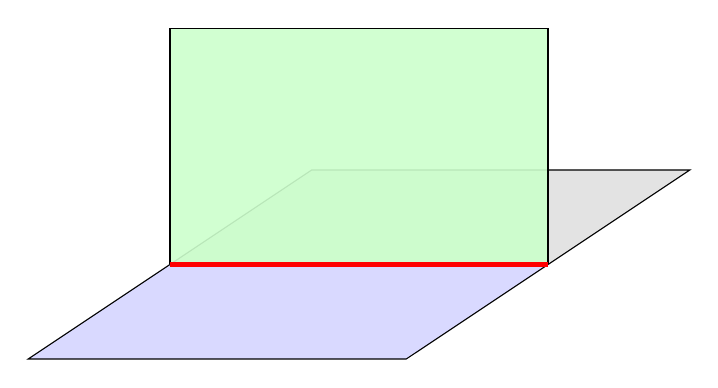
\begin{tikzpicture}[
    scale=1.2,
    % Define a 3D-like perspective by setting the coordinate vectors.
    % x goes to the right, y goes up, and z gives a sense of depth.
    z={(-0.6cm,-0.4cm)}, 
    x={(1cm,0cm)},      
    y={(0cm,1cm)}       
]
    % --- Define Coordinates for the vertices of the book ---
    
    % The spine is a 1-cell from O to A
    \coordinate (O) at (0,0,0);
    \coordinate (A) at (4,0,0);

    \coordinate (B_Back) at (4,0,-2.5);
    \coordinate (C_Back) at (0,0,-2.5);

    \coordinate (B_Front) at (4,0,2.5);
    \coordinate (C_Front) at (0,0,2.5);

    \coordinate (B_Up) at (4,2.5,0);
    \coordinate (C_Up) at (0,2.5,0);

    % Draw book pages
    \fill[gray!30, opacity=0.75] (O) -- (A) -- (B_Back) -- (C_Back) -- cycle;
    \draw (O) -- (C_Back) -- (B_Back) -- (A);

    \fill[blue!20, opacity=0.75] (O) -- (A) -- (B_Front) -- (C_Front) -- cycle;
    \draw (O) -- (C_Front) -- (B_Front) -- (A);

    \fill[green!20, opacity=0.9] (O) -- (A) -- (B_Up) -- (C_Up) -- cycle;
    \draw (O) -- (C_Up) -- (B_Up) -- (A);

    % --- Draw the Spine on top so it stands out ---
    \draw[line width=1.5pt, red] (O) -- (A);
\end{tikzpicture}
\caption{A 3-page book}
\label{fig:threepagebook}
\end{figure}

% It would make so much more sense if we excluded the covers of the book when counting the pages.
% Then, a book with more than 0 pages is not homeomorphic to a surface. 
% However, this would be an annoying substitution in later proofs.
\begin{defn}
    An \(n\)-page book is a collection of \(n\) \(2\)-cubes each glued along a common edge.
    This edge is called the spine of the book.
\end{defn}

Books are common structures found in configuration spaces.
One goal for this project is to determine which configuration spaces are surfaces.

\begin{thm}
A book with more than \(2\) pages is not a surface.
\end{thm}
\begin{proof}
Suppose there exists an \(n\)-page book that is a surface but \(n > 2\).
Let \(p\) be some point in the interior of the book's spine.
% pg. 225 Munkres states that an m-manifold X is a Hausdorff space such that for each point x in 
% X there exists a nehiborhood of x that is homeomorphic to an open subset of R^m.
% Let U be the neihborhood of p in X, V be the open subset of R^2, and \phi
% be the homeomorphism from U to V.
% Take some open disk B centered at \phi(p) in V such that \closure{B} \subseteq V
% restrict \phi to this open disk (this is okay to do in the codomain as \phi is a bijection).
Since the book is homeomorphic to a surface, there exists an open neighborhood \(U\) of \(p\)
which is homeomorphic to an open disk \(B\) in \(\mathbb{R}^2\).
Let \(\phi\) be a homeomorphism from \(\closure{U}\) to \(\closure{B}\) and \(S\) be the portion of book's spine inside of \(U\).
Notice that \(U \setminus S\) consists of \(n\) path components--one from each page of the book.
However,
\[
U\setminus S \cong \phi(U\setminus S) = B \setminus \phi(S).
\]

We claim that \(\phi(S)\) must separate \(B\) into two components.
To see this, first note that \(\phi(S)\) is a properly imbedded arc in \(B\) with \(\Bd(\phi(S))\) consisting of two
points on \(\Bd(B)\).
% homemorphisms map boundary points to boundary points, interior points to interior points, and exterior points to exterior points.
% This is common knowledge but a proof might be necessary TODO.
Since \(\Bd(B)\) is homeomorphic to a circle, there exists two different paths \(\alpha\) and \(\beta\) 
connecting these two points together (See Figure \ref{fig:thm:book_1_1}).

\begin{figure}[h!]
    \centering
    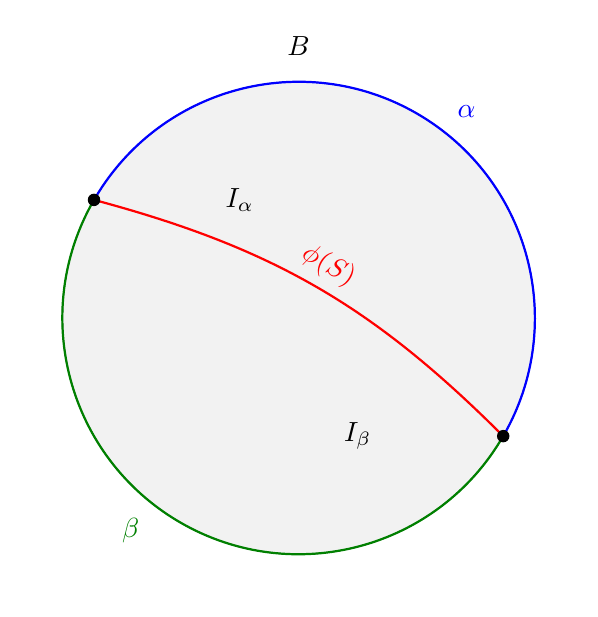
\begin{tikzpicture}[scale=1.5]
        % Define the main circle (the disk D^2) and fill it lightly
        \fill[gray!10] (0,0) circle (2cm);
        \draw (0,0) circle (2cm);
        \node at (0, 2.3) {\(B\)};

        % Define the start and end points of the arc on the boundary of the disk
        \coordinate (P1) at (150:2cm);
        \coordinate (P2) at (-30:2cm);

        % Draw the separating arc phi(S \cap U) with a distinct color
        \draw[thick, red] (P1) to[bend left=15] node[above, pos=0.5, sloped] {\(\phi(S)\)} (P2);

        % Draw the boundary path alpha
        \draw[thick, blue] (P2) arc (-30:150:2cm);
        \node[blue, above, xshift=18pt, yshift=-5pt] at (60:2cm) {\(\alpha\)};
        
        % Draw the boundary path beta
        \draw[thick, green!50!black] (P1) arc (150:330:2cm);
        \node[green!50!black, below, xshift=-18pt, yshift=5pt] at (240:2cm) {\(\beta\)};
        
        % Label the two regions separated by the arc
        \node at (-0.5, 1) {\(I_{\alpha}\)};
        \node at (0.5, -1) {\(I_{\beta}\)};
        
        % Mark the endpoints on the boundary
        \fill (P1) circle (1.5pt);
        \fill (P2) circle (1.5pt);

    \end{tikzpicture}
    \caption{The arc \(\phi(S)\) separates the open disk \(B\) into two components, \(I_{\alpha}\) and \(I_{\beta}\).}
    \label{fig:thm:book_1_1}
\end{figure}

The Jordan curve theorem guarantees that the simple closed curve \(\alpha \cup \phi(S)\) (resp. \(\beta \cup \phi(S)\))
separate \(B \setminus (\alpha \cup \phi(S))\) (resp. \(B \setminus (\beta \cup \phi(S))\)) into a bounded connected component
\(I_{\alpha}\) and an unbounded connected component \(O_{\alpha}\) (resp. \(I_{\beta}\) and \(O_{\beta}\)) when imbedded in \(\mathbb{R}^2\).
Notice \(B\setminus \phi(S) = I_{\alpha} \cup I_{\beta}\).
Since \(I_{\alpha} \subseteq O_{\beta}\) and \(I_{\beta} \cap O_{\beta} = \emptyset\),
we have that \(I_{\alpha} \cap I_{\beta} = \emptyset\).
So, \(I_{\alpha}\) and \(I_{\beta}\) form a separation of \(B\setminus \phi(S)\).
\end{proof}

Another common structure found found in graph configuration spaces are \(n\)-cubes.
Consider the graph in Figure \ref{fig:3edges} and imagine \(3\) particles placed at \(u_1\), \(v_1\), and \(w_1\).
Each particle can simultaneously move to \(u_2\), \(v_2\), and \(w_2\) resulting in \(3\)-cube in the configuration space (see Figure \ref{fig:3cube}).

\begin{figure}[h!]
    \centering
\begin{tikzpicture}
    \node (u1) at (0, 2) {\(u_1\)};
    \node (u2) at (0, 0) {\(u_2\)};
    \draw (u1) -- (u2);
    \node (v1) at (2, 2) {\(v_1\)};
    \node (v2) at (2, 0) {\(v_2\)};
    \draw (v1) -- (v2);
    \node (w1) at (4, 2) {\(w_1\)};
    \node (w2) at (4, 0) {\(w_2\)};
    \draw (w1) -- (w2);
\end{tikzpicture}
    \caption{Three edges}
    \label{fig:3edges}
\end{figure}

\begin{figure}[h!]
    \centering
    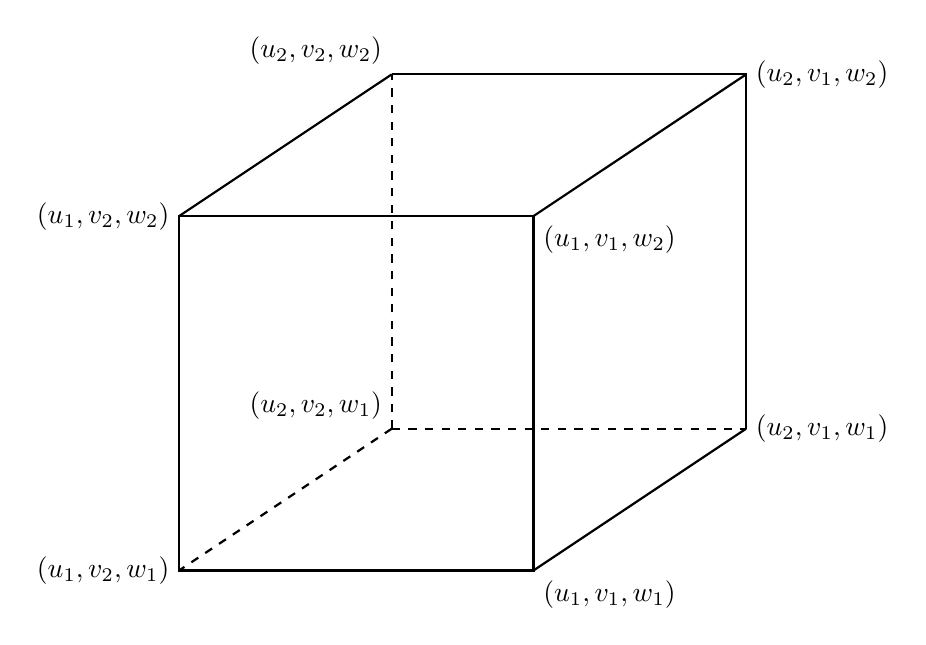
\begin{tikzpicture}[
    scale=1.5,
    % Define a 3D-like perspective by setting the coordinate vectors.
    % x goes to the right, y goes up, and z gives a sense of depth.
    x={(1cm,0cm)},
    y={(0cm,1cm)},
    z={(-0.6cm,-0.4cm)}
]
    % --- Style Definitions ---
    % Define styles for the cube's edges to make the code cleaner.
    % 'visible' edges are solid and thick.
    % 'hidden' edges are dashed and thick.
    \tikzstyle{visible} = [draw, thick, black]
    \tikzstyle{hidden} = [draw, thick, dashed, black]

    % --- Vertex Coordinates ---
    % Define the 8 vertices of the cube using (x,y,z) coordinates.
    % The side length of the cube is 3 units.
    \def\s{3}
    \coordinate (A) at (0,0,0);
    \coordinate (B) at (\s,0,0);
    \coordinate (C) at (\s,\s,0);
    \coordinate (D) at (0,\s,0);
    \coordinate (E) at (0,0,\s);
    \coordinate (F) at (\s,0,\s);
    \coordinate (G) at (\s,\s,\s);
    \coordinate (H) at (0,\s,\s);

    % --- Draw Hidden Edges ---
    % Draw the edges that would be obscured from view first. These are the
    % edges connected to the rearmost vertex (A).
    \draw[hidden] (A) -- (B);
    \draw[hidden] (A) -- (D);
    \draw[hidden] (A) -- (E);

    % --- Draw Visible Edges ---
    % Draw the visible edges on top of the hidden ones.
    \draw[visible] (B) -- (C) -- (D);
    \draw[visible] (E) -- (F) -- (G) -- (H) -- cycle;
    \draw[visible] (B) -- (F);
    \draw[visible] (C) -- (G);
    \draw[visible] (D) -- (H);

    % --- Optional: Label Vertices ---
    % Uncomment the following lines to add labels to each vertex.
    \node at (A) [above left] {\((u_2, v_2, w_1)\)};
    \node at (B) [right] {\((u_2, v_1, w_1)\)};
    \node at (C) [right] {\((u_2, v_1, w_2)\)};
    \node at (D) [above left] {\((u_2, v_2, w_2)\)};
    \node at (E) [left] {\((u_1, v_2, w_1)\)};
    \node at (F) [below right] {\((u_1, v_1, w_1)\)};
    \node at (G) [below right] {\((u_1, v_1, w_2)\)};
    \node at (H) [left] {\((u_1, v_2, w_2)\)};    
\end{tikzpicture}
\caption{3-cube}
\label{fig:3cube}
\end{figure}

Visually \(n\)-cubes are ``clearly'' not surfaces when \(n > 2\).
However, we can show this formally with an argument using the fundamental group.
\begin{thm}
\(n\)-cubes are not surfaces when \(n > 2\).
\end{thm}
\begin{proof}
    Suppose an \(n\)-cube \(C\) is a surface for some \(n > 2\).
    % imbed C in R^n
    Pick some point \(p\) in the interior of \(C\).
    Since \(C\) is a surface there exists some open ball \(B^n(p, \epsilon)\) in the interior of \(C\) such that 
    it is centered at \(p\) and is homeomorphic to some open neighborhood \(V\) of \(\mathbb{R}^2\).
    Let \(q\) be the point in \(V\) corresponding to \(p\).
    
    % TODO just use the fact that local simple connectedness fails after removing a point in D^2 but doesn't after removing a point in S^2.
\end{proof}

Books and cubes are the meat and potatos of the coming proofs.
\section{Computing the Euler characteristic of graph configuration spaces}
To compute the euler characteristic of an unorderd \(n\) point graph configuration space we need to count
for each \(0 \le k \le n\) the number of \(k\)-cubes present.

A \(k\) cube exists if and only if \(k\) particles are free to move simultaneously while \(n - k\)
particles remain fixed.
Hence the general formula for the number of \(k\) cubes in \(\DUConf_n(\Gamma)\) is
\[
    \abs{\phi(k)} \cdot\binom{\abs{V(\Gamma)} - 2k}{n - k}
\]
where \(\phi(k)\) defined as follows.

\begin{defn}
\(\phi(k)\) is the collection consisting of all unordered sets of exactly \(k\) disjoint edges in \(\Gamma\)
where \(\phi(0) = \{\emptyset\}\).
\end{defn}

Note that we define \(\phi(0) = \{\emptyset\}\) so that \(\abs{\phi(0)} = 1\).
With this definition, \(\abs{\phi(k)}\) is also known as the number of ``\(k\)-matchings'' in \(\Gamma\).

We now express the Euler characteristic of \(\DUConf_n(\Gamma)\) in the following lemma.
\begin{lem}
\label{lem:eulercharacteristic}
\[
\chi(\DUConf_n(\Gamma)) = \sum_{k=0}^{n} (-1)^k \abs{\phi(k)} \binom{\abs{V(\Gamma)} - 2k}{n - k}
\]
\end{lem}

Counting the number of \(k\)-matchings for small graphs can be done efficiently 
with a simple sweep over all \(k\) combinations of edges.
We have done this for several small graphs (see Figure \ref{fig:euler_characteristics}) that are relevant in later chapters.
\begin{figure}[h!]
\centering
\begin{tabular}{c | c | c}
   \(\Gamma\) & \(n\) & \(\chi(\DUConf_n(\Gamma))\) \\
   \hline
   \(K_5\) & 2 & -5 \\
   \(K_{3,3}\) & 2 & -3 \\
   \(K_5\) & 3 & -5 \\
   \(\Theta_4\) & 3 & -4 \\
   \(K_{3,3}\) & 4 & -3
\end{tabular}
\caption{Euler characteristic of certain unordered graph configuration spaces.}
\label{fig:euler_characteristics}
\end{figure}
% TODO add a link to the code that computes these values.

% TODO read/cite Mark Jerrum's paper "Two-dimensional monomer-dimer systems are computationally intractable"
% where he proves computing the matching polynomial for planar graphs is P# ?
In general, for larger graphs this computation quickly becomes unwieldly.
A workaround for this computational challenge is determining the Euler characteristic of certain classes of graphs.
In \cite{appiah2024algebraicstructurehyperbolicgraph} the \textit{pulsar graph} was defined.
See Figure \ref{fig:pulsargraph} for a depiction of the pulsar graph \(\mathcal{P}_{m,n_1,n_2}\).

\begin{figure}[h!]
    \centering
\begin{tikzpicture}[scale=1]
    % Define the two main suspension vertices, positioned closer together
    \node (a1) at (0, 1) {\(a_1\)};
    \node (a2) at (0, -1) {\(a_2\)};

    % Define the intermediate vertices for the 'm' paths
    \node (b1) at (-1, 0) {\(b_1\)};
    \node (bm) at (1, 0) {\(b_m\)};
    \node at (0,0) {\(\dots\)};

    % Draw the edges for the 'm' paths, passing through the b_i nodes
    \draw (a1) to[out=180, in=90] (b1);
    \draw (b1) to[out=270, in=180] (a2);

    \draw (a1) to[out=0, in=90] (bm);
    \draw (bm) to[out=270, in=0] (a2);

    % Define vertices for the 'n1' rays attached to a1, spread out as in the drawing
    \node (c1) at (-1, 2) {\(c_1\)};
    \node (c1p) at (-2, 3) {\(c'_1\)};
    \node (cn1) at (1, 2) {\(c_{n_1}\)};
    \node (cn1p) at (2, 3) {\(c'_{n_1}\)};
    \node at (0, 2.5) {\(\dots\)};

    % Draw edges for the 'n1' rays
    \draw (a1) -- (c1);
    \draw (c1) -- (c1p);
    \draw (a1) -- (cn1);
    \draw (cn1) -- (cn1p);

    % Define vertices for the 'n2' rays attached to a2, also spread out
    \node (d1) at (-1, -2) {\(d_1\)};
    \node (d1p) at (-2, -3) {\(d'_1\)};
    \node (dn2) at (1, -2) {\(d_{n_2}\)};
    \node (dn2p) at (2, -3) {\(d'_{n_2}\)};
    \node at (0, -2.5) {\(\dots\)};

    % Draw edges for the 'n2' rays
    \draw (a2) -- (d1);
    \draw (d1) -- (d1p);
    \draw (a2) -- (dn2);
    \draw (dn2) -- (dn2p);
\end{tikzpicture}
\caption{The Pulsar graph \(\mathcal{P}_{m,n_1,n_2}\)}
\label{fig:pulsargraph}
\end{figure}

\begin{thm}
    \label{thm:pulsargrapheuler}
    The Euler characteristic of \(\DUConf_{3}(\mathcal{P}_{m,n_1,n_2})\) is
    \[
    \frac{m^{3}}{6} - \frac{3 m^{2}}{2} - \frac{m n_{1}^{2}}{2} - \frac{3 m n_{1}}{2} - \frac{m n_{2}^{2}}{2} - \frac{3 m n_{2}}{2} + \frac{7 m}{3} - \frac{n_{1}^{3}}{3} + \frac{7 n_{1}}{3} - \frac{n_{2}^{3}}{3} + \frac{7 n_{2}}{3}.
    \]
\end{thm}
\begin{proof}
Since there are no \(k\)-cubes when \(k > 3\), ``all'' we need to do is compute the number of \(k\)-matchings
for \(k = 0, 1, 2, 3\).
We introduce some terminology to make the counting easier.
An ``outer emission edge'' is one of the edges \(c_i c_i'\) or \(d_i d_i'\).
An ``inner emission edge'' is one of the edges \(a_1 c_i\) or \(a_2 d_i\).
A ``middle edge'' is one of the edges \(a_1 b_i\) or \(a_2 b_i\).
We then count the number of matching by considering edges taken from each of these three categories.


\textbf{3-matchings}
The following table summarizes the computations for each case.

\begin{center}
\begin{tabular}{c | c | c | c | c }
Subcase & Outer & Inner & Middle & Count \\ 
\hline
1 & 3 & 0 & 0 & \(\binom{n_1 + n_2}{3}\) \\
2 & 2 & 1 & 0 & \((n_1 + n_2)\binom{n_1 + n_2 - 1}{2}\) \\
3 & 2 & 0 & 1 & \(2m\binom{n_1 + n_2}{2}\) \\
4 & 1 & 2 & 0 & \(n_1n_2(n_1 + n_2 - 2)\) \\
5 & 1 & 1 & 1 & \(m n_2 (n_1 + n_2 - 1) + m n_1 (n_1 + n_2 - 1)\) \\
6 & 1 & 0 & 2 & \(m(m-1)(n_1 + n_2)\) \\
7 & 0 & 3 & 0 & 0 \\
8 & 0 & 2 & 1 & 0 \\
9 & 0 & 1 & 2 & 0 \\
10 & 0 & 0 & 3 & 0 
\end{tabular}
\end{center}

We elaborate on each of these cases below.
\begin{enumerate}
    \item All three edges are chosen from the outer emission edges.
    There are \(\binom{n_1 + n_2}{3}\) such matchings.

    \item One edge is chosen from the \(n_1 + n_2\) inner emission edges,
    and two edges are chosen from the outer emission edges. Since there are \(n_1 + n_2 - 1\)
    outer emission edges disjoint from the chosen inner emission edge,
    there are \((n_1 + n_2)\binom{n_1 + n_2 - 1}{2}\) total such matchings.

    \item One edge is chosen from the \(2m\) middle edges, and two edges are chosen from the outer emission edges.
    Since there are \(n_1 + n_2\) outer emission edges disjoint from the chosen middle edge,
    there are \( 2m\binom{n_1 + n_2}{2} \) such matchings.

    \item Two edges are chosen from the \(n_1 + n_2\) inner emission edges, and one edge is chosen from the outer emission edges.
    Since the only way to chose two disjoint inner emission edges is to choose one from the \(n_1\) edges
    attached to \(a_1\) and one from the \(n_2\) edges attached to \(a_2\),
    there are \(n_1 n_2\) such choices.
    After choosing two inner emission edges, there are \(n_1 + n_2 - 2\) outer emission edges disjoint from the chosen inner emission edges.


    \item One edge is chosen from a middle edge, one edge is chosen from an inner emission edge, and one edge is chosen from an outer emission edge.
    If we pick one of the \(n_1\) top inner emission edges, there are \(m\) middle edges disjoint from it, and \((n_1 + n_2 - 1)\)
    outer emission edges disjoint from both the chosen inner emission edge and middle edge.
    Similarly, if we pick one of the \(n_2\) bottom inner emission edges,
    there are \(m\) middle edges disjoint from it, and \((n_1 + n_2 - 1)\)
    outer emission edges disjoint from both the chosen inner emission edge and middle edge.


    \item Two edges are chosen from the middle edges, and one edge is chosen from the outer emission edges.
    After choosing one of the top \(m\) middle edges, there are \(m - 1\) disjoint middle edges remaining.
    This accounts for all ways to choose to disjoint pairs of middle edges.
    Since there are \(n_1 + n_2\) outer emission edges disjoint from any middle edge,
    there are \(m (m - 1) (n_1 + n_2)\) such matchings.
\end{enumerate}

\textbf{2-matchings:}
The following table summarizes the computations for each case.
\begin{center}
\begin{tabular}{c | c | c | c | c }
Subcase & Outer & Inner & Middle & Count \\
\hline
1 & 2 & 0 & 0 & \(\binom{n_1 + n_2}{2}\) \\
2 & 1 & 1 & 0 & \( (n_1 + n_2) (n_1 + n_2 - 1) \) \\
3 & 1 & 0 & 1 & \( 2m (n_1 + n_2) \) \\
4 & 0 & 2 & 0 & \( n_1 n_2 \) \\
5 & 0 & 1 & 1 & \( m n_2 + m n_1 \) \\
6 & 0 & 0 & 2 & \( m (m - 1)\)
\end{tabular}
\end{center}
Again, we elaborate on each of these cases below.
\begin{enumerate}
    \item Both edges are chosen from the outer emission edges. There are \(\binom{n_1 + n_2}{2}\) such matchings.
    \item Choose one of the \((n_1 + n_2)\) inner emission edges, then there are \((n_1 + n_2 - 1)\) possible disjoint outer emission edges.
    \item Choose one of the \(2m\) middle edges, then there are \((n_1 + n_2)\) possible disjoint outer emission edges.
    \item Choose one of the \(n_1\) top inner emission edges, then there are \(n_2\) bottom possible disjoint inner emission edges.
    \item If we choose one of the \(m\) top middle edges, then there are \(n_2\) possible bottom disjoint inner emission edges.
    Similarly, if we choose one of the \(m\) bottom middle edges, then there are \(n_1\) possible top disjoint inner emission edges.
    \item Choose one of the \(m\) top middle edges, then there are \((m-1)\) possible disjoint bottom middle edges.
\end{enumerate}

\textbf{1-matchings:}
This case is much more straightforward. We simply add up the number of ways to select one edge from each of the three categories.
Hence the total number of 1-matchings is
\[
(n_1 + n_2) + (n_1 + n_2) + 2m
\]

\textbf{0-matchings:}
There is exactly one 0-matching, the empty set.


\textbf{Final Count}
Now that we know the number of \(k\)-matchings for \(k = 0, 1, 2, 3\), we can compute the Euler characteristic
with the formula from Lemma \ref{lem:eulercharacteristic}.
The simplification was not done by hand, but rather with the help of a computer algebra system namely SymPy.
% TODO add a link to the code used.
\end{proof}

\begin{rem}
Substituting in \(n_1 = 0\) and \(n_2 = 0\) the pular graph becomes \(\Theta_m\) aka. \(K_{2,m}\).
So, 
the euler characteristic of \(\DUConf_3(\Theta_m)\) is
\[
\frac{m^{3}}{6} - \frac{3 m^{2}}{2} + \frac{7 m}{3}
\]
This aligns with results in section 4 of \cite{appiah2024algebraicstructurehyperbolicgraph}.
\end{rem}
\chapter{Manifolds}
% Input sections
\section{Background}
In his thesis \cite{abrams2000configurationspaces}, Abrams asked:
For which \(n\) and \(\Gamma\) is \(\DConf_n(\Gamma)\) homeomorphic to a closed manifold?
He establishes a partial answer to this question in Corollary 5.8: 
if \(\Gamma\) is a connected graph
without loops and \(\DConf_n(\Gamma)\) is homeomorphic to a closed
\(n\)-dimensional manifold, then either \(n = 1\) and \(\Gamma\) is a cycle, or
\(n = 2\) and \(\Gamma\) is \(K_5\) or \(K_{3,3}\).

Advised by Peter Haskell, Praphat Fernandes in his undergraduate thesis
demonstrates that if \(\Gamma\) is a simple graph and \(\DConf_2(\Gamma)\)
is a \(2\)-psuedomanifold without boundary the following are true.
\begin{enumerate}
    \item If \(\Gamma\) contains a valence 4 vertex, then \(\Gamma\) is \(K_5\).
    \item If every vertex in \(\Gamma\) has valence 3, then \(\Gamma\) is \(K_{3,3}\).
\end{enumerate}
This recovers Abrams' result about when \(\DConf_2(\Gamma)\) 
is a \(2\)-manifold, as Praphat also shows that
if \(\Gamma\) is simple and \(\DConf_2(\Gamma)\) is a 2-psuedomanifold without boundary,
then the valence of every vertex in \(\Gamma\) is between 3 and 4,
and \(\DConf_2(\Gamma)\) is a 2-manifold. Also advised by Peter Haskell, Molly Ison in \cite{ison2005two} 
extends Fernandes' work in her masters thesis to 2-psuedomanifolds with boundary.

In Example 4.3 in \cite{ko2012characteristics}, it is shown that \(\DConf_3(\Theta_4)\)
is a closed orientable surface of genus 3 by computing its fundamental group and using the
fact that discretized configuration spaces are \(K(\pi, 1)\) spaces.
This result is recovered in \cite{appiah2024algebraicstructurehyperbolicgraph}
with a strictly combinatorial argument.

In correspondance wit Abrams, him and a prior student of his
looked in detail at ``level \(j\)-psuedomanifolds''.
A level \(j\)-psuedomanifold is a CW complex where the interior of every cell of codimension \(k\)
is a manifold point for \(0 \le k \le j\).
With this definition, a level \(n\)-psuedomanifold is a \(n\)-manifold 
and every \(n\)-complex is a level \(0\)-psuedomanifold.
They showed that if \(\Gamma\) is a colored graph then \(\DConf_n(\Gamma)\) is a level \(2\)-psuedomanifold
if and only if \(\Gamma\) is a ``colored cover'' of \(K_{2n+1}\) or \(K_{n+1, n+1}\).
Moreover, they show that find that there are no level \(3\)-psuedomanifolds of the form \(\DConf_n(\Gamma)\)
when \(n > 2\).
It follows there are no \(n\)-manifolds of the form \(\DConf_n(\Gamma)\) when \(n > 2\).


\section{A Long List of Lemmas}
From this point forward in the section we assume that \(\DConf_n(\Gamma)\) is an \(m\)-manifold without boundary
and \(M\) is an \((m-1)\)-matching in \(\Gamma\).

\subsection{Minimum Graph Size and Key Lemma}

\begin{lem}
\label{lem:graph-size}
    \(\Gamma\) has at least \(m + n\) vertices and \(n \ge m\).
\end{lem}

\begin{proof}
    If \(\Gamma\) has less than \(n\) vertices, then \(\DConf_n(\Gamma)\) is empty;
    so, suppose \(\Gamma\) has at least \(n\) vertices.
    If \(\Gamma\) has less than \(n + m\) vertices, then
    for any configuration of \(n\) particles on \(\Gamma\)
    at most \(m-1\) particles can simultaneously move.
    Since exactly \(m\) particles need to be able to simultaneously move for an \(m\)-cube 
    to exist in \(\DConf_n(\Gamma)\), no configuration in \(\DConf_n(\Gamma)\)
    can have a neighborhood homeomorphic to an open set in \(\mathbb{R}^m\).

    Similarly, if \(n < m\), then there are not enough particles that can simultaneously move
    for an \(m\)-cube to exist in \(\DConf_n(\Gamma)\). So, \(n \ge m\). 
\end{proof}

This next lemma is the key to all following proofs.
The idea is that if we have an \((m-1)\)-cube in the configuration space,
then there needs to be exactly two \(m\)-cubes that border it for the points
in that \((m-1)\)-cube to look locally like \(\mathbb{R}^m\).

\begin{lem}
    \label{lem:special-edges}
    For any collection \(\mathcal{V}\) of \(n - (m - 1)\) vertices in \(\Gamma - V(M)\), there exists exactly \textbf{two}
    edges \(e_1\) and \(e_2\) in \(\Gamma - V(M)\) that are incident to vertices in \(\mathcal{V}\)
    and vertices not in \(\mathcal{V}\).

    Furthermore, these edges \(e_1\) and \(e_2\) satisfy all of the following conditions.
    \begin{enumerate}[label=(\roman*)]
    \item \(e_1\) and \(e_2\) are both incident to one vertex in \(\mathcal{V}\)
    \item \(e_1\) and \(e_2\) are both incident to one vertex not in \(\mathcal{V}\)
    \item \(e_1\) and \(e_2\) share exactly one common vertex.
    \end{enumerate}

    Equivalently, exactly one of the following hold in Figure \ref{fig:lem:special-edges}
    \begin{figure}[h!]
        \centering
        \begin{enumerate*}[label=(\arabic*)]
            \item \label{fig:lem:manifolds_1_1}
            \begin{minipage}{.3\textwidth}
                \centering
                \(v_1 \in \mathcal{V}\) \textit{and} \(w_1, w_2 \not \in \mathcal{V}\) \\
                \vspace{1em}
                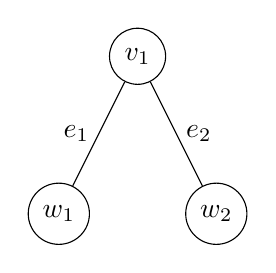
\begin{tikzpicture}
                    \node (v1) at (3, 2) [circle, draw] {\(v_1\)};
                    \node (w1) at (2, 0) [circle, draw] {\(w_1\)};
                    \node (w2) at (4, 0) [circle, draw] {\(w_2\)};

                    \draw (v1) -- (w1) node[midway, left] {\(e_1\)};
                    \draw (v1) -- (w2) node[midway, right] {\(e_2\)};
                \end{tikzpicture} 
            \end{minipage}

            \hspace{3em}

            \item \label{fig:lem:manifolds_1_2}
            \begin{minipage}{.3\textwidth}
                \centering
                \(v_1, v_2 \in \mathcal{V}\) \textit{and} \(w_1 \not \in \mathcal{V}\) \\
                \vspace{1em}
                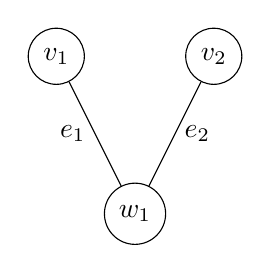
\begin{tikzpicture}
                    \node (v1) at (2, 2) [circle, draw] {\(v_1\)};
                    \node (v2) at (4, 2) [circle, draw] {\(v_2\)};
                    \node (w1) at (3, 0) [circle, draw] {\(w_1\)};

                    \draw (v1) -- (w1) node[midway, left] {\(e_1\)};
                    \draw (v2) -- (w1) node[midway, right] {\(e_2\)};
                \end{tikzpicture}
            \end{minipage}
        \end{enumerate*}
        \caption{Lemma \ref{lem:special-edges} possibilities.}
        \label{fig:lem:special-edges}
    \end{figure}
\end{lem}

\begin{proof}
    Let \(\mathcal{V}\) be a collection of \(n - (m - 1)\) vertices in \(\Gamma - V(M)\)
    and \(p\) be the configuration of \(n\) particles placed on \(\Gamma\) such that
    \(n - (m - 1)\) particles are placed at each vertex in \(\mathcal{V}\)
    and \(m - 1\) particles on each edge in \(M\).
    
    As the particles move move along the edges in \(M\), an \((m-1)\)-cube containing \(p\)
    is spanned in \(\DConf_n(\Gamma)\).
    Since the configuration space is an \(m\)-manifold without boundary, 
    this \((m-1)\)-cube must border exactly two distinct \(m\)-cubes.
    For this \((m-1)\)-cube to border two \(m\)-cubes,
    there needs to exist \textbf{two} additional mutually exclusive particle movements.
    Let \(v_1, v_2 \in \mathcal{V}\) and \(w_1, w_2 \not \in \mathcal{V}\) be the vertices corresponding
    to the origins and destinations of these additional particle movements.
    If \(v_1 \neq v_2\) and \(w_1 \neq w_2\), then two particles would be able to move simultaneously
    resulting in an \((m+1)\)-cube being spanned in \(\DConf_n(\Gamma)\) contradicting 
    that it is an \(m\)-manifold.
\end{proof}

\subsection{\(m = 1\) or No Cycles}

\begin{lem}
    \label{lem:manifold-max-degree}
    Every vertex in \(\Gamma - V(M)\) has degree at most \(3\).
\end{lem}

\begin{proof}
    Suppose \(\Gamma - V(M)\) has a vertex \(v\) with degree greater than \(3\).
    We proceed by cases on \(n\).

    \textbf{Case 1:} \(n \le m - 1 + \deg(v)\)
    In the context of Lemma \ref{lem:special-edges},
    construct \(\mathcal{V}\) so that all \(n - (m - 1) = n - m + 1\)
    vertices are on the vertices adjacent to \(v\).
    Then, there are too many edges with one endpoint in \(\mathcal{V}\)
    and other outside of \(\mathcal{V}\) for Lemma \ref{lem:special-edges} to hold.

    \textbf{Case 2:} \(n > m - 1 + \deg(v)\)
    Lemma \ref{lem:graph-size} guarantees that \(\Gamma - V(M)\) has at least
    \(n + m - 2(m - 1) = n - m + 2\) vertices.
    So, \(\abs{V(\Gamma - V(M))} > \deg(v) + 1\).
    More importantly, it's clear now that we can now construct a \(\mathcal{V}\)
    so that it contains \(v\) and every vertex adjacent to \(v\).
    By Lemma \ref{lem:special-edges}, there is at least one vertex \(w \not \in \mathcal{V}\).
    Let \(\mathcal{V}' = \left(\mathcal{V}\setminus\{v\}\right)\cup\{w\}\) i.e. 
    swap out \(v\) for \(w\) in \(\mathcal{V}\).
    Then, again there are now too many edges with one endpoint in \(\mathcal{V}'\)
    and another outside of \(\mathcal{V}'\) to for Lemma \ref{lem:special-edges} to hold.
\end{proof}

\begin{lem}
    \label{lem:manifold-is-claw}
    If \(\Gamma - V(M)\) contains a degree \(3\) vertex,
    then \(\Gamma - V(M) \cong K_{1,3}\) and \(n = m + 1\).
\end{lem}

\begin{proof}
    Suppose \(\Gamma - V(M)\) contains a degree \(3\) vertex \(v\).
    First we show that \(n\) must be equal to \(m + 1\) by considering two cases.

    \textbf{Case 1:} \(n > m + 1\)
    % TODO Clean up
    Fill up the \(Y\)-graph.
    There must be at least one free vertex.
    Put a particle there instead of at \(v\)
    Book.

    \textbf{Case 2:} \(n < m + 1\)
    In this case \(n\) must equal \(m\) by Lemma \ref{lem:graph-size}.
    Let \(\mathcal{V}\) consist of just the vertex \(v\).
    Then, there are too many edges with one endpoint in \(\mathcal{V}\)
    and another outside of \(\mathcal{V}\) to for Lemma \ref{lem:special-edges} to hold.
    Namely, the three edges incident to \(v\).

    Now we show that there cannot be any other vertices in \(\Gamma - V(M)\) besides \(v\) and its neighbors.
    Suppose there was a vertex \(w \neq v\) in \(\Gamma - V(M)\) that is not adjacent to \(v\).
    Let \(\mathcal{V} = \{v, w\}\).
    Then, again there are too many edges with one endpoint in \(\mathcal{V}\)
    and another outside of \(\mathcal{V}\) to for Lemma \ref{lem:special-edges} to hold.
    Namely, the three edges incident to \(v\).

    Finally, we show that there cannot be any edges in \(\Gamma - V(M)\)
    besides the three edges incident to \(v\).

    Suppose there was another edge \(e\) in \(\Gamma - V(M)\) not incident to \(v\) and
    let \(a\) and \(b\) be the vertices incident to \(e\) and \(c\) be the other vertex adjacent to \(v\)
    (see Figure \ref{fig:lem:manifold-is-claw-1}).

    \begin{figure}
        \centering
        \begin{tikzpicture}
            \node (v) at (0,0) [circle, draw] {\(v\)};
            \node (a) at (-2,-2) [circle, draw] {\(a\)};
            \node (b) at (2,-2) [circle, draw] {\(b\)};
            \node (c) at (0,2) [circle, draw] {\(c\)};

            \draw (v) -- (a);
            \draw (v) -- (b);
            \draw (v) -- (c);
            \draw (a) -- (b) node[midway, below] {\(e\)};
        \end{tikzpicture}
        \caption{\(\Gamma - V(M)\) with an extra edge \(e\)}
        \label{fig:lem:manifold-is-claw-1}
    \end{figure}

    Let \(\mathcal{V} = \{a, c\}\).
    Then, again there are too many edges with one endpoint in \(\mathcal{V}\) and another outside of \(\mathcal{V}\).
    Namely, \(cv\), \(av\), and \(bv\).

    Therefore \(\Gamma - V(M)\) must consist solely of \(v\), its neighbors, and the edges incident to \(v\).
\end{proof}

\begin{lem}
    If \(m = 1\), then \(\Gamma \cong K_{1,3}\) and \(n = 2\),
    or \(\Gamma\) is one or more cycles and \(n \in \{1, \abs{V(\Gamma)} - 1\}\) 
\end{lem}

\begin{proof}
    It is sufficient to show that the degree of every vertex in \(\Gamma\) is exactly \(2\).
    Let \(v\) be some vertex in \(\Gamma\). By Lemma \ref{lem:graph-size}, there exists \(n\) other vertices in \(\Gamma\).
    The edges \(e_1\) and \(e_2\) guaranteed by Lemma \ref{lem:special-edges} must then both be incident to \(v\)
    and there can be no other edges incident to \(v\) and these \(n\) vertices.
    If there were another edge incident to \(v\), then \(v\) would have degree at least \(3\)
    meaning \(\Gamma\) would have to be \(K_{1,3}\).
    So, then \(n = 2\) and \(\Gamma\) is just \(K_{1,3}\).

    Otherwise, \(v\) has degree exactly \(2\).
    Since \(v\) was arbitrary, every vertex in \(\Gamma\) has degree exactly \(2\)
    meaning, \(\Gamma\) is one or more cycles.
    If \(1 < n < \abs{V(\Gamma)} - 1\), then there are too many ways for particles to move.
\end{proof}

Now that the \(m = 1\) case is completely determined, we only consider when \(m \ge 2\) from this point onward.

\begin{lem}
    \(\Gamma - V(M)\) must be \(K_{1,3}\) or contains a cycle.
\end{lem}

\begin{proof}
    % TODO rephrase as to no use particle placement language
    Suppose that \(\Gamma - V(M)\) contains no vertices of degree 3 nor any cycles.
    Then \(\Gamma - V(M)\) is a forest whose trees are paths.
    Since \(\Gamma - V(M)\) has at least \(m + n - 2(m - 1) = n - m + 2\) vertices by Lemma \ref{lem:graph-size},
    we can place \(n - (m - 1)\) particles filling up the paths.
    Then there is only one edge contradicting Lemma \ref{lem:special-edges}.
\end{proof}

\subsection{\(m > 1\) and Cycles}
Since we know what happens when \(m = 1\) or \(\Gamma - V(M)\) contains no cycles.
Continue to assume that \(m > 1\) but now also suppose \(\Gamma - V(M)\) contains a cycle \(C\).

\begin{lem}
    \label{lem:cycle-length-1}
    If \(n > m\), then \(C\) has length at most \(n - m + 2\).
\end{lem}

\begin{proof}
    By Lemma \ref{lem:graph-size} \(\Gamma - V(M)\) has at least \(n + m - 2(m - 1) = n - m + 2\) vertices.
    So, after picking any \(n - (m - 1) = n - m + 1\) vertices, there must be at least one other vertex in \(\Gamma - V(M)\).

    Suppose \(C\) had more than \(n - m + 2\) vertices.
    Since \(n > m\), it follows that \(n - m + 2 \ge 3\) and that \(C\) has at least \(4\) vertices.
    So, after picking \(n - m + 1\) vertices in a path on \(C\), there are still at least \(2\) vertices left on \(C\)
    contradicting Lemma \ref{lem:special-edges}.
\end{proof}

\begin{lem}
    If \(n > m\) and \(C\) has length \(n - m + 2\),
    then \(\Gamma - V(M) = C\).
\end{lem}

\begin{proof}
    Suppose there was another vertex \(v\) in \(\Gamma - V(M) - V(C)\).
    Then, after picking this vertex and \(n - m\) vertices on \(C\),
    there are two vertices left on \(C\) contradicting Lemma \ref{lem:special-edges}.
\end{proof}

\begin{lem}
    If \(n > m\), then \(n = (m-1) + \abs{V(C)} - 1\)
\end{lem}

\begin{proof}
    Notice that 
    Lemma \ref{lem:cycle-length-1} guarantees \(\abs{V(C)} \le n - m + 2\).
    So, \((m - 1) + \abs{V(C)} - 1 \le n\).
    Suppose \((m - 1) + \abs{V(C)} - 1 < n\).
    We proceed by cases on the number of vertices in \(\Gamma - V(M)\).
    Lemma \ref{lem:graph-size} guarantees that \(\Gamma - V(M)\) has at least
    \(n + m - 2(m - 1) = n - m + 2\) vertices.


    % 1 free vertex case
    \textbf{Case 1:} \(\Gamma - V(M)\) has exactly \(n - m + 2\) vertices.
    % Should get that \Gamma - V(M) is a bunch of cycles

    % > 1 free vertices
    \textbf{Case 2:} \(\Gamma - V(M)\) has more than \(n - m + 2\) vertices.
    % This should be an easy contradiction as we can just move two particles off of C
    % onto 2 free vertices


\end{proof}

\begin{lem}
    If \(n > m\), then \(\Gamma - V(M)\) has at most \(4\) vertices.
\end{lem}

\begin{proof}
    Suppose \(\Gamma - V(M)\) has more than \(4\) vertices.
    We proceed by cases on the length of \(C\).

    \textbf{Case 1:} \(C\) has length \(3\)

    \begin{figure}[h!]
        \centering
        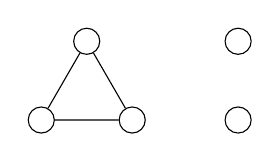
\begin{tikzpicture}
            \node (v1) at (0,0) [circle, draw] {};
            \node (v2) at (1.155,0) [circle, draw] {};
            \node (v3) at (0.577,1) [circle, draw] {};
            \draw (v1) -- (v2) -- (v3) -- (v1);

            \node (v4) at (2.5, 0) [circle, draw] {};
            \node (v5) at (2.5, 1) [circle, draw] {};
        \end{tikzpicture}
    \caption{\(C\) and two other vertices}
    \end{figure}

    Two subcases.

    First subcase.
    \begin{figure}[h!]
        \centering
        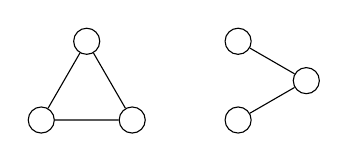
\begin{tikzpicture}
            \node (v1) at (0,0) [circle, draw] {};
            \node (v2) at (1.155,0) [circle, draw] {};
            \node (v3) at (0.577,1) [circle, draw] {};
            \draw (v1) -- (v2) -- (v3) -- (v1);

            \node (v4) at (2.5, 0) [circle, draw] {};
            \node (v5) at (2.5, 1) [circle, draw] {};
            \node (v6) at (3.366, 0.5) [circle, draw] {};
            \draw (v4) -- (v6) -- (v5);
        \end{tikzpicture}
    \end{figure}

    Second subcase.
    \begin{figure}[h!]
        \centering
        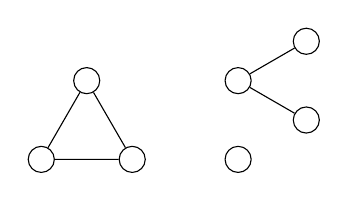
\begin{tikzpicture}
            \node (v1) at (0,0) [circle, draw] {};
            \node (v2) at (1.155,0) [circle, draw] {};
            \node (v3) at (0.577,1) [circle, draw] {};
            \draw (v1) -- (v2) -- (v3) -- (v1);

            \node (v4) at (2.5, 0) [circle, draw] {};
            \node (v5) at (2.5, 1) [circle, draw] {};
            \node (v6) at (3.366, 0.5) [circle, draw] {};
            \node (v7) at (3.366, 1.5) [circle, draw] {};
            \draw (v6) -- (v5) -- (v7);

        \end{tikzpicture}
    \end{figure}

    \textbf{Case 2:} \(C\) has length \(4\)

    \begin{figure}[h!]
        \centering
        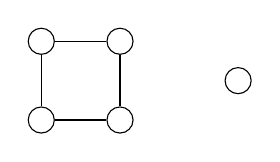
\begin{tikzpicture}
            \node (v1) at (0, 0) [circle, draw] {};
            \node (v2) at (1, 0) [circle, draw] {};
            \node (v3) at (1, 1) [circle, draw] {};
            \node (v4) at (0, 1) [circle, draw] {};
            \draw (v1) -- (v2) -- (v3) -- (v4) -- (v1);

            \node (v5) at (2.5, 0.5) [circle, draw] {};

        \end{tikzpicture}
    \end{figure}

    \textbf{Case 3:} \(C\) has length greater than \(5\) --
    Cleverly change which matching we choose and we can get a degree \(3\) vertex.

    \begin{figure}[h!]
        \centering
        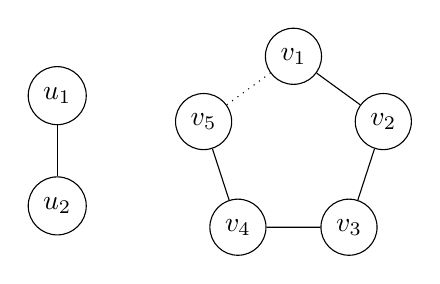
\begin{tikzpicture}
        \foreach \i in {1,...,5} \node (v\i) at ({162-72*\i}:1.2) [circle, draw] {\(v_{\i}\)};
        \draw (v1) -- (v2) -- (v3) -- (v4) -- (v5);

        \draw[dotted] (v5) -- (v1);

        \node (u1) at (-3,.7) [circle, draw] {\(u_1\)};
        \node (u2) at (-3,-.7) [circle, draw] {\(u_2\)};
        \draw (u1) -- (u2);
        \end{tikzpicture}
    \end{figure}

    \begin{figure}[h!]
        \centering
        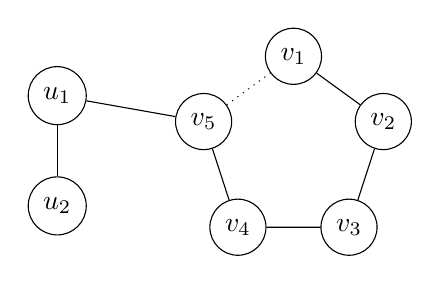
\begin{tikzpicture}
        \foreach \i in {1,...,5} \node (v\i) at ({162-72*\i}:1.2) [circle, draw] {\(v_{\i}\)};
        \draw (v1) -- (v2) -- (v3) -- (v4) -- (v5);

        \draw[dotted] (v5) -- (v1);

        \node (u1) at (-3,.7) [circle, draw] {\(u_1\)};
        \node (u2) at (-3,-.7) [circle, draw] {\(u_2\)};
        \draw (u1) -- (u2);

        \draw (u1) -- (v5);
        \end{tikzpicture}
    \end{figure}

\end{proof}

\begin{lem}
If \(n > m\) and \(C\) has length \(3\), then \(\Gamma - V(M) \cong K_3\) or \(\Gamma - V(M) \cong K_3 \cup K_1\).
\end{lem}

\begin{proof}
    Since \(\Gamma - V(M)\) cannot have more than \(4\) vertices and also contains \(C\),
    then either \(\Gamma - V(M)\) is just \(C\) or \(C\) and another isolated vertex.

    In the later case, this isolated vertex cannot be connected to \(C\) otherwise
    we would have a degree \(3\) vertex.
\end{proof}

\begin{lem}
If \(n > m\) and \(C\) has length \(4\), then \(\Gamma - V(M) \cong K_{2,2}\)
\end{lem}

\begin{proof}
Since \(\Gamma - V(M)\) contains \(C\) and has at most \(4\) vertices,
\(\Gamma - V(M)\) is just \(C\) which isomorphic to \(K_{2,2}\).
\end{proof}


Abrams already studied the case when \(n = m\) in detail but we analyze it here for completeness.
\begin{lem}
If \(n = m\), then \(\Gamma - V(M)\) has at most \(4\) vertices.
\end{lem}

\begin{proof}
    Suppose \(\Gamma - V(M)\) has more than \(4\) vertices.
    This argument is similar to the \(n > m\) case where we proceed by cases on the length of \(C\).

    \textbf{Case 1:} \(C\) has length \(3\).

    \textbf{Case 2:} \(C\) has length \(4\).

    \textbf{Case 3:} \(C\) has length greater than \(4\).

\end{proof}

\begin{lem}
If \(n = m\) and \(C\) has length \(3\), then \(\Gamma - V(M) \cong K_3\).
\end{lem}

\begin{lem}
If \(n = m\) and \(C\) has length \(4\), then \(\Gamma - V(M) \cong K_{2,2}\).
\end{lem}



\section{Exclusivity of Subgraphs}

Now that we have determined the possible subgraphs \(\Gamma - V(M)\) for some \((m-1)\)-matching \(M\),
we claim that if \(\Gamma - V(M_0) \cong \Lambda\) for some \((m-1)\)-matching \(M_0\) and subgraph \(\Lambda\),
then \(\Gamma - V(M) \cong \Lambda\) for any \((m-1)\)-matching \(M\).

\begin{thm}
    Suppose \(\Conf_n(\Gamma)\) is an \(m\)-manifold without boundary for \(m \ge 2\),
    then there exists a subgraph \(\Lambda\) in \(\Gamma\)
    such that \(\Lambda \in \{K_3, K_{2,2}, K_3 \cup K_1, K_{1,3}\}\)
    and \(\Gamma - V(M) \cong \Lambda\) for any \((m-1)\)-matching \(M\) in \(\Gamma\).
\end{thm}

\begin{proof}
If \(\Lambda\) is \(K_{2,2}\) then \(n\) can be \(m\) or \(m + 2\).
In either case we cannot have that \(\Gamma - V(M) \cong K_{1,3}\) or \(\Gamma - V(M) \cong K_3 \cup K_1\)
since \(n\) must be \(m + 1\) there.
Furthermore, we cannot have that \(\Gamma - V(M) \cong K_3\) while \(\Lambda \cong K_{2,2}\)
since that would imply the number of vertices in \(\Gamma\) is different in each case.
So, \(K_{2,2}\) cannot occur simultaneously with any of the other subgraphs.

Similarly, \(K_3\) cannot occur simultaneously with \(K_{1,3}\) or \(K_3 \cup K_1\)
since the number of vertices in \(\Gamma\) would total up to different amounts.

So, we just need to show that \(K_{1,3}\) and \(K_3 \cup K_1\) cannot occur simultaneously.
% TODO 

\end{proof}

\section{Theorems}

\begin{thm}
  Let \(m \ge 2\). If \(\DConf_n(\Gamma)\) is an \(m\)-manifold without boundary, 
  then \(\DConf_n(\Gamma)\) is one of the following.
\begin{enumerate}
  \item \(\DConf_m(K_{2m+1}) \cong \DConf_{m+1}(K_{2m+1})\)
  \item \(\DConf_m(K_{m+1, m+1}) \cong \DConf_{m+2}(K_{m+1, m+1})\)
  \item \(\DConf_{m+1}(K_{2m + 1} \cup K_1)\)
  \item \(\DConf_{m+1}(K_{m, m+2})\)
\end{enumerate}
\end{thm}

\begin{proof}
  Let \(M\) be an \((m-2)\) matching in \(\Gamma\).
  As shown in the previous section, \(\Gamma - N(M)\) is a unique subgraph of \(\Gamma\).
  So, as shown in the previous section there are \(5\) possible \((n - (m-2), \Gamma - N(M))\) pairs.
  \begin{enumerate}
    \item If \((n - (m - 2), \Gamma - N(M)) = (2, K_5)\), 
    then \(n\) must be \(m\) and 
    by Lemma \ref{lem:complete-graph-is-special}, \(\Gamma\) must be \(K_{2m+1}\).

    \item If \((n - (m - 2), \Gamma - N(M)) = (3, K_5)\), 
    then \(n\) must be \(m + 1\) and
    by Lemma \ref{lem:complete-graph-is-special}, \(\Gamma\) must be \(K_{2m+1}\).

    \item If \((n - (m - 2), \Gamma - N(M)) = (2, K_{3,3})\), 
    then \(n\) must be \(m\) and
    by Lemma \ref{lem:bipartite-graph-is-special}, \(\Gamma\) must be \(K_{m+1, m+1}\).

    \item If \((n - (m - 2), \Gamma - N(M)) = (4, K_{3,3})\), 
    then \(n\) must be \(m + 2\) and
    by Lemma \ref{lem:bipartite-graph-is-special}, \(\Gamma\) must be \(K_{m+1, m+1}\).

    \item If \((n - (m - 2), \Gamma - N(M)) = (3, K_{2,4})\), 
    then \(n\) must be \(m + 1\) and
    by Lemma \ref{lem:bipartite-graph-is-special}, \(\Gamma\) must be \(K_{m, m+2}\).

  \end{enumerate}
\end{proof}

In \cite{abrams2000configurationspaces}, Abrams showed the following.
\begin{prop}
If \(m > 2\) then \(\DConf_m(K_{(m+1), (m+1)})\) and \(\DConf_{m}(K_{(2m+1)})\) are not \(m\)-manifolds.
\end{prop}
Applying his duality theorem, it follows that
\(\DConf_{m+1}(K_{m+1, m+1})\) and \(\DConf_{m+1}(K_{2m+1})\)
are not \(m\) manifolds either.
\input{chapters/manifolds/special-graphs.tex}
\chapter{PL Morse Theory}
\section{Background}

This is a modified proof of a statement in \cite{appiah2024algebraicstructurehyperbolicgraph}.
\begin{thm}
\label{thm:descendinglinks}
Let \(X\) be a finite cubical complex,
\(f: X \rightarrow \mathbb{R}\) be a PL Morse function,
and \([a,b]\) be contained in the image of \(f\). 
For any \(c\) in the open interval \((a,b)\), if
\begin{enumerate}
    \item \(f^{-1}([a,c])\) is connected.
    \item \(f^{-1}((c,b))\) contains no vertices.
    \item \(f^{-1}(\{b\})\) is a set of vertices.
    \item The descending links of each vertex \(v\) in \(f^{-1}(\{b\})\) 
        is homotopically equivalent to \(n_v\) distinct points.
\end{enumerate}
then, \(f^{-1}[[a,b]]\) is homotopy equivalent to a wedge of \(f^{-1}[[a,c]]\)
with exactly \(\displaystyle r = \sum_{v \in f^{-1}(\{b\})} (n_v - 1)\) circles and consequently
\(\pi_1(f^{-1}[[a,b]]) = \pi_1(f^{-1}[a,c])\,*\,\mathbb{F}_r\)
where \(\mathbb{F}_r\) is a free group on \(r\) generators.
\end{thm}

\begin{proof}
We first consider the case when there is only one vertex \(v\) in \(f^{-1}(\{b\})\).
Let the descending link of \(v\) be the disjoint spaces \(\{A_1, ..., A_{n_v}\}\). 

By Proposition 2.7 in \cite{Bestvina2008PL}, \(f^{-1}([c,b])\) is homotopically equivalent
rel \(f^{-1}(\{a\})\) to the cone on the descending links of \(v\) attached to \(v\). 

Since \(f^{-1}([a,c])\) is path connected, 
we can find paths from a point in each \(A_i\) to some \(p\) in \(f^{-1}(\{c\}) \cap A_1\).
Let \(Q\) be the union of the cone and these paths.

% Visually this next line is clear but I should say more.
Notice \(Q\) homotopically equivalent to a wedge of \(n_v - 1\) circles.

Since each added path in \(Q\) contracts to \(p\), we can retract \(Q \cap f^{-1}([a,c])\) to \(p\).

% I should be more explicit about how the fundamental group of the intersection is null homotopic
% and how \pi_1 of a wedge of circles is just a free group on how many circles there are.
The Seifert-Van Kampen theorem guarantees that \(\pi_1(f^{-1}([a,b]))\) is just \(\pi_1(f^{-1})([a,c]) * \mathbb{F}_{n_v - 1}\).

When there are multiple points in \(f^{-1}(\{b\})\), as mentioned in \cite{Bestvina2008PL}
the cones on each point \(v \in f^{-1}(\{b\})\) get attached to each \(v\) in a pairwise disjoint fashion.
Similar to before, by finding paths through \(f^{-1}([a,c])\) we can connect together each cone
resulting in a wedge of \(r = \sum_{v} (n_v - 1)\) circles.
The Seifert-Van Kampen theorem then guarantees that
\(\pi_1(f^{-1}([a,b])) = \pi_1(f^{-1}([a,c])) * \mathbb{F}_r\).

\end{proof}
\input{chapters/pl-morse-theory/pulsar-graph.tex}

% --- Used in abstract.tex to get the length of the thesis ---
\label{LastPage}

% --- Bibliography ---
{
    \singlespacing
    \bibliographystyle{abbrv}
    \bibliography{bibliography}
}
\end{document}